% =====================================================================
%  Informe TP N.º 2 - I206 Inferencia y Estimación - UdeSA
%  Grupo 01. Cifras tomadas de la ejecución completa de resolucion.ipynb.
%  Compilar desde esta carpeta (las figuras se leen de figures/):
%      tectonic TP2_G01.tex        o        pdflatex TP2_G01.tex
% =====================================================================
\documentclass[11pt,a4paper]{article}

\usepackage[utf8]{inputenc}
\usepackage[T1]{fontenc}
\usepackage{lmodern}
\usepackage[spanish,es-tabla,es-nodecimaldot,es-noquoting]{babel}
\usepackage{amsmath,amssymb}
\usepackage{graphicx}
\usepackage[a4paper,margin=2.2cm]{geometry}
\usepackage{booktabs}
\usepackage{float}
\usepackage{placeins}
\usepackage[font=small,labelfont=bf,skip=4pt]{caption}
\usepackage{enumitem}
\usepackage{fancyhdr}
\usepackage{microtype}
\usepackage[hidelinks]{hyperref}

\graphicspath{{figures/}}

% ---------------------- Datos del grupo ---------------------------
\newcommand{\grupo}{1}
\newcommand{\legajoAlsina}{370833}
\newcommand{\legajoBunge}{370842}
\newcommand{\legajoDietrich}{370913}
\newcommand{\profesores}{Copa, Débora; Carducci, Leonardo; García Gulisano Pau}
% ------------------------------------------------------------------

\newcommand{\E}{\mathbb{E}}
\newcommand{\Prob}{\mathbb{P}}
\newcommand{\MI}{I(X;X')}
\newcommand{\img}[1]{\texttt{img\_#1}}

\setlength{\parskip}{0.25em}
\clubpenalty=10000
\widowpenalty=10000
\setlist{itemsep=0.15em, topsep=0.25em}
\setlength{\textfloatsep}{10pt plus 2pt minus 2pt}
\setlength{\floatsep}{8pt plus 2pt minus 2pt}
\setlength{\intextsep}{8pt plus 2pt minus 2pt}

\pagestyle{fancy}
\fancyhf{}
\lhead{Inferencia y Estimación}
\rhead{Trabajo Práctico N.\textsuperscript{o} 2 -- Grupo \grupo}
\cfoot{\thepage}
\setlength{\headheight}{14pt}

\begin{document}

% =====================================================================
%  Carátula
% =====================================================================
\begin{titlepage}
  \centering
  \vspace*{1cm}
  {\Large Universidad de San Andrés\par}
  \vspace{0.3cm}
  {\large Ingeniería en Inteligencia Artificial\par}
  \vspace{0.3cm}
  {\large I206 -- Inferencia y Estimación\par}
  \vspace{3cm}
  {\Huge\bfseries Trabajo Práctico N.\textsuperscript{o} 2\par}
  \vspace{0.8cm}
  {\LARGE Compresión de imágenes sin pérdida\\[0.2cm] mediante codificación de Huffman\par}
  \vspace{0.5cm}
  {\large Codificación píxel a píxel, codificación diferencial e información mutua\par}
  \vspace{3cm}
  {\large\bfseries Grupo \grupo\par}
  \vspace{0.5cm}
  {\large
  \begin{tabular}{l@{\hspace{1.5cm}}l}
    Bautista Alsina & Legajo \legajoAlsina \\[0.15cm]
    Santos Bunge    & Legajo \legajoBunge \\[0.15cm]
    Hans Dietrich   & Legajo \legajoDietrich \\
  \end{tabular}\par}
  \vspace{1.5cm}
  {\large Profesores: \profesores\par}
  \vfill
  {\large Primavera 2026\par}
\end{titlepage}

% =====================================================================
\section*{Resumen}
Se comparan dos formas de comprimir tres imágenes en escala de grises con Huffman: codificar las
intensidades y codificar las diferencias entre píxeles vecinos. Se estiman sus distribuciones,
entropías e información mutua, y se comprueba que los bits promedio medidos coinciden con la
longitud media calculada. Los residuos mejoran la compresión de las dunas y la partitura, pero
empeoran la de la textura de arena. Como experimento adicional, se mezclan los píxeles de las dunas:
la codificación directa cuesta lo mismo, mientras que la de residuos pierde su ventaja. También se
implementan un compresor y un descompresor de archivos binarios.

% =====================================================================
\section{Introducción}
% =====================================================================
Una imagen en escala de grises de 8 bits almacena cada intensidad con la misma cantidad de bits.
Cuando los niveles aparecen con frecuencias diferentes, un código de longitud variable puede reducir
el promedio de bits por píxel. Huffman permite construir un código libre de prefijo que minimiza ese
promedio para una distribución dada.

El objetivo del trabajo es comparar esa codificación directa con la de los residuos entre vecinos.
En regiones suaves, las diferencias pequeñas son frecuentes y pueden necesitar menos bits que las
intensidades. Se estudian tres imágenes para comprobar cuándo ocurre esta mejora y relacionarla con
la dependencia espacial mediante información mutua. En ambos esquemas se verifica la recuperación
exacta de la imagen en escala de grises.

% =====================================================================
\section{Marco teórico y metodología}
% =====================================================================
\paragraph{Entropía y código de Huffman.}
Sea $X$ una fuente discreta con masa de probabilidad $p(x)$. Su entropía en bits,
$H(X) = -\sum_x p(x)\log_2 p(x)$, es una cota inferior de la longitud media de un código binario
símbolo a símbolo unívocamente decodificable~\cite{shannon,cover}. Aquí $H(X)$ es marginal: para
aprovechar la dependencia entre píxeles se necesita otra representación o un modelo con contexto. Un código asigna a cada símbolo una palabra de $l(x)$ bits y su
longitud media es $L = \sum_x p(x)\,l(x)$. El algoritmo de Huffman~\cite{huffman} construye el
código libre de prefijo de menor $L$ para una pmf dada. Con al menos dos símbolos de probabilidad
positiva cumple $H(X) \le L < H(X) + 1$. En general no alcanza exactamente la entropía porque las
longitudes son enteras; sí la alcanza para probabilidades diádicas $p(x)=2^{-l(x)}$. Por ejemplo,
dos símbolos equiprobables tienen $H=L=1$. Si hay un único símbolo, nuestra implementación usa la
palabra \texttt{0} para conservar la cantidad de ocurrencias al decodificar con la función provista:
entonces $H=0$ y $L=1$, una excepción a la cota estricta por la convención de palabra no vacía.
Con una fuente de $M$ símbolos usados vale además $H(X)\le\log_2 M$, con igualdad
solo si son equiprobables.

\paragraph{Estimación empírica.}
Tratamos cada píxel como una realización de la fuente $X$ y estimamos la pmf por frecuencia
relativa, $\hat p(x) = n_x / N$, donde $n_x$ es la cantidad de píxeles con intensidad $x$ y $N$ el
total de píxeles. Es el histograma de 256 bins normalizado; bajo un modelo categórico i.i.d. coincide
con el estimador de máxima verosimilitud de la pmf~\cite{teoricas}. Todas las entropías del trabajo se calculan sobre estas estimaciones, sumando
solo sobre los símbolos con $\hat p(x) > 0$.

\paragraph{Codificación diferencial.}
Recorremos la imagen en \emph{serpentina}: la fila 0 de izquierda a derecha, la fila 1 de derecha a
izquierda, y así sucesivamente. De este modo la imagen de $M \times N$ píxeles queda como una única
secuencia $x_1, \dots, x_{MN}$ en la que cada píxel es vecino espacial del anterior, y basta con
guardar un único píxel inicial $x_1$ con sus 8 bits. El resto se representa con los residuos
$y_k = x_k - x_{k-1}$, que toman valores en $\{-255, \dots, 255\}$, y la imagen se reconstruye de
forma exacta con $x_k = x_{k-1} + y_k$, es decir, con la suma acumulada de los residuos a partir de
$x_1$. Elegimos este recorrido frente al de guardar el primer píxel de cada fila porque el costo fijo
baja de $8M$ bits a 8 y porque deja toda la imagen como una sola fuente $Y$. La contrapartida es que un
error en un residuo se propagaría a todos los píxeles siguientes y no solo al resto de la fila.

\paragraph{Información mutua.}
Para cuantificar la dependencia entre vecinos llamamos $X'$ al píxel anterior y $X$ al actual,
tomando exactamente los mismos pares $(x_{k-1}, x_k)$ que generan los residuos. La información mutua
\[
\MI = \sum_{x,x'} \hat p(x,x') \log_2 \frac{\hat p(x,x')}{\hat p(x)\,\hat p(x')}
     = H(X) + H(X') - H(X,X')
\]
mide cuántos bits de incerteza sobre un píxel se eliminan al conocer su vecino~\cite{cover,teoricas2}.
La pmf conjunta se estima con el histograma bidimensional de $256 \times 256$ bins. Conocido $X'$,
la transformación $Y=X-X'$ es invertible, de modo que $H(Y\mid X')=H(X\mid X')$. Como condicionar
no aumenta la entropía, $H(Y)\ge H(X\mid X')$. De estas relaciones se obtiene
\[
H(X)-H(Y)=\MI-I(Y;X').
\]
Así, $\MI$ acota la reducción de entropía respecto del modelo marginal, pero no garantiza que la
resta la consiga: depende de la información que conserve el residuo sobre el vecino. La comparación
entre longitudes Huffman también incluye las redundancias de ambos códigos; el costo por píxel y el
del archivo agregan el inicial y los metadatos correspondientes.
Las marginales de esta sección se calculan sobre las secuencias de los pares, que tienen $MN-1$
muestras ($X'$ omite el último píxel y $X$ el primero), para que los tres términos de la identidad
usen las mismas muestras. Difieren de la $H(X)$ de la Sección~\ref{sec:ej1} en un solo píxel y
coinciden en todas las cifras mostradas.

\paragraph{Implementación.}
Las tres imágenes provistas (Figura~\ref{fig:imagenes}) vienen en color; las convertimos a escala de
grises de 8 bits antes de todo el análisis, así que ``sin pérdida'' se refiere siempre a esa versión.
Los ejercicios 1 a 3 están en un único cuaderno que reutiliza las mismas funciones de estimación de
pmf, entropía y compresión para intensidades y para residuos; las funciones de construcción y
decodificación del código de Huffman son las provistas por la cátedra~\cite{tp2}. En cada compresión
se decodifica la cadena de bits y se verifica que la imagen reconstruida coincide píxel a píxel con la
original. Las cifras citadas en este informe son las que imprime el cuaderno.

\begin{figure}[H]
  \centering
  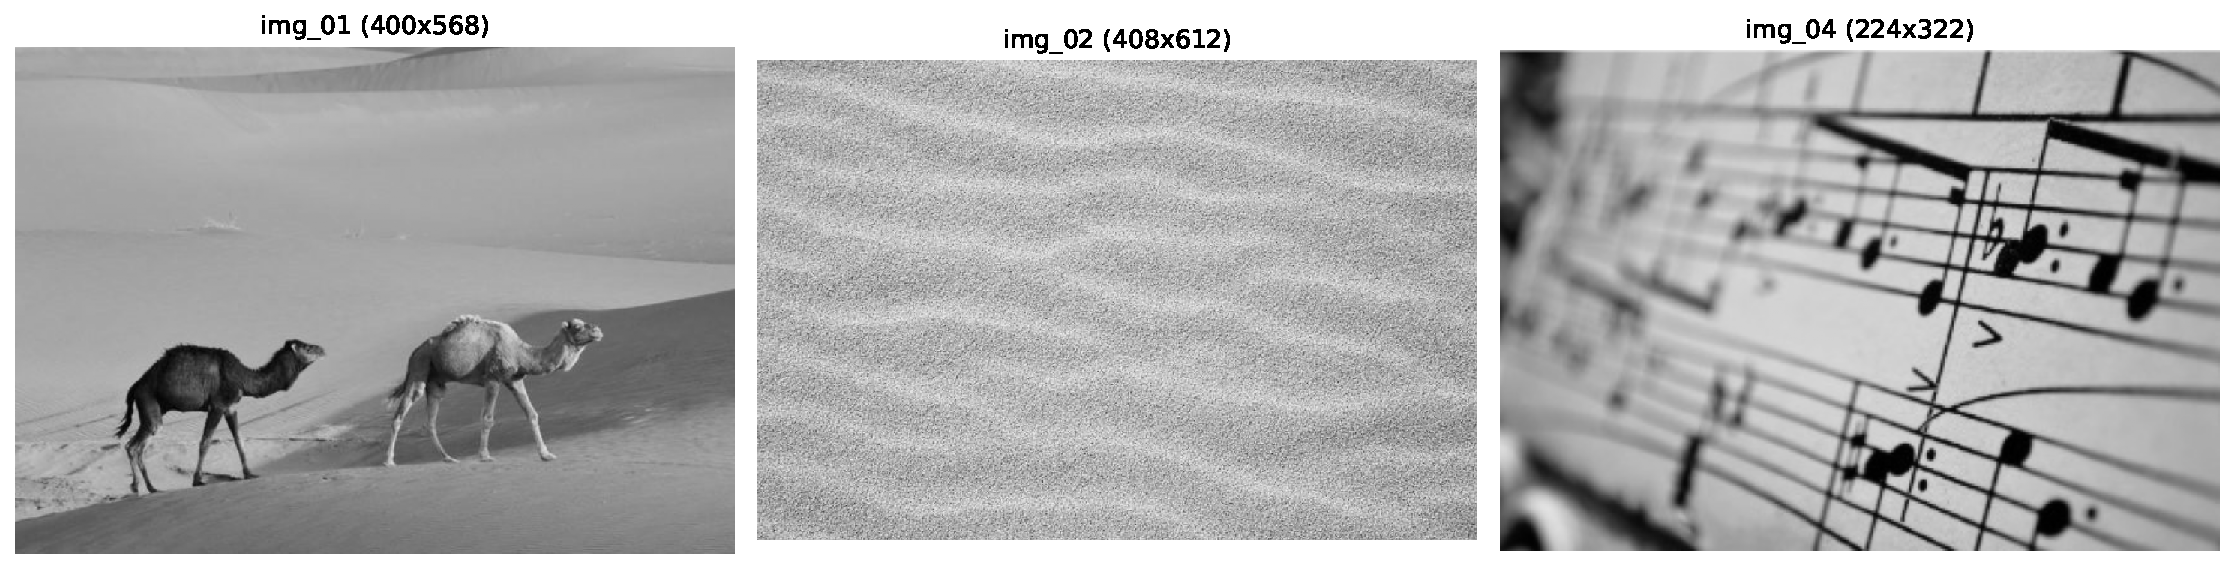
\includegraphics[width=0.92\textwidth]{imagenes}
  \caption{Las tres imágenes en escala de grises, con sus dimensiones. \img{01}: dunas con camellos,
  grandes regiones suaves. \img{02}: textura de arena de grano fino. \img{04}: partitura
  fotografiada, con fondo claro de brillo gradual, zonas desenfocadas y trazos oscuros.}
  \label{fig:imagenes}
\end{figure}

% =====================================================================
\section{Ejercicio 1: codificación píxel a píxel}
\label{sec:ej1}
% =====================================================================
\paragraph{Masa de probabilidad y entropía (inciso a).}
La fila superior de la Figura~\ref{fig:pmf} muestra $\hat p(x)$ para cada imagen y la
Tabla~\ref{tab:ej1} resume las entropías. Las tres imágenes usan una cantidad parecida de niveles de
gris (entre 205 y 228 de los 256 posibles), con cotas $\log_2 M$ entre 7.68 y 7.83 bits;
 la diferencia de entropía está en cómo se reparte la masa dentro de ese
rango. \img{01} tiene un pico muy marcado alrededor de 165 (el tono de la arena de las dunas) y
otro menor en 100, con poca masa fuera de ellos, y por eso su entropía es la más baja. \img{02} usa
menos niveles pero los reparte de forma acampanada y bastante pareja entre 120 y 240. \img{04}
tiene la pmf más plana: una meseta entre 0 y 150 correspondiente a la tinta y las sombras, y una
zona densa entre 150 y 220 para el fondo, lo que cubre casi todo el rango y da la entropía más alta.

\begin{table}[H]
  \centering
  \caption{Codificación píxel a píxel. Niveles usados, entropía, longitud media teórica $L$ del código
  de Huffman, bits promedio medidos sobre la cadena comprimida y tasa de compresión respecto de 8 bits.}
  \label{tab:ej1}
  \begin{tabular}{lrrrrrr}
    \toprule
    Imagen & Píxeles & Niveles & $H(X)$ [bits] & $L$ [bits] & Bits/píxel medidos & $8/L$ \\
    \midrule
    \img{01} & 227\,200 & 224 & 6.281 & 6.310 & 6.310 & 1.27 \\
    \img{02} & 249\,696 & 205 & 6.783 & 6.809 & 6.809 & 1.17 \\
    \img{04} &  72\,128 & 228 & 7.138 & 7.165 & 7.165 & 1.12 \\
    \bottomrule
  \end{tabular}
\end{table}

\paragraph{Compresión con Huffman (inciso b).}
Con la pmf estimada construimos el código de Huffman, codificamos cada píxel y concatenamos las
palabras. Los bits promedio por píxel de la cadena resultante coinciden exactamente con la longitud
media teórica $L$ (Tabla~\ref{tab:ej1}), como corresponde: al reemplazar $\hat p(x) = n_x/N$ en
$L = \sum_x \hat p(x)\, l(x)$ se obtiene $\frac{1}{N}\sum_x n_x\, l(x)$, que es la cantidad total de
bits dividida por $N$. La comparación sirve como verificación de consistencia entre la implementación
y la teoría. En las tres imágenes se cumple $H(X) \le L < H(X) + 1$ y la redundancia $L - H(X)$ es de
apenas 0.03 bits, muy por debajo del bit de margen que garantiza la cota.

La compresión frente a los 8 bits por píxel es modesta: la tasa $8/L$ va de 1.12 a 1.27, es decir,
un ahorro de entre el 11\,\% y el 21\,\%. Como Huffman ya está prácticamente en el límite $H(X)$,
el margen para mejorar un código por intensidad es pequeño. La codificación diferencial del
siguiente ejercicio permite aprovechar parte de la estructura espacial.

\begin{figure}[H]
  \centering
  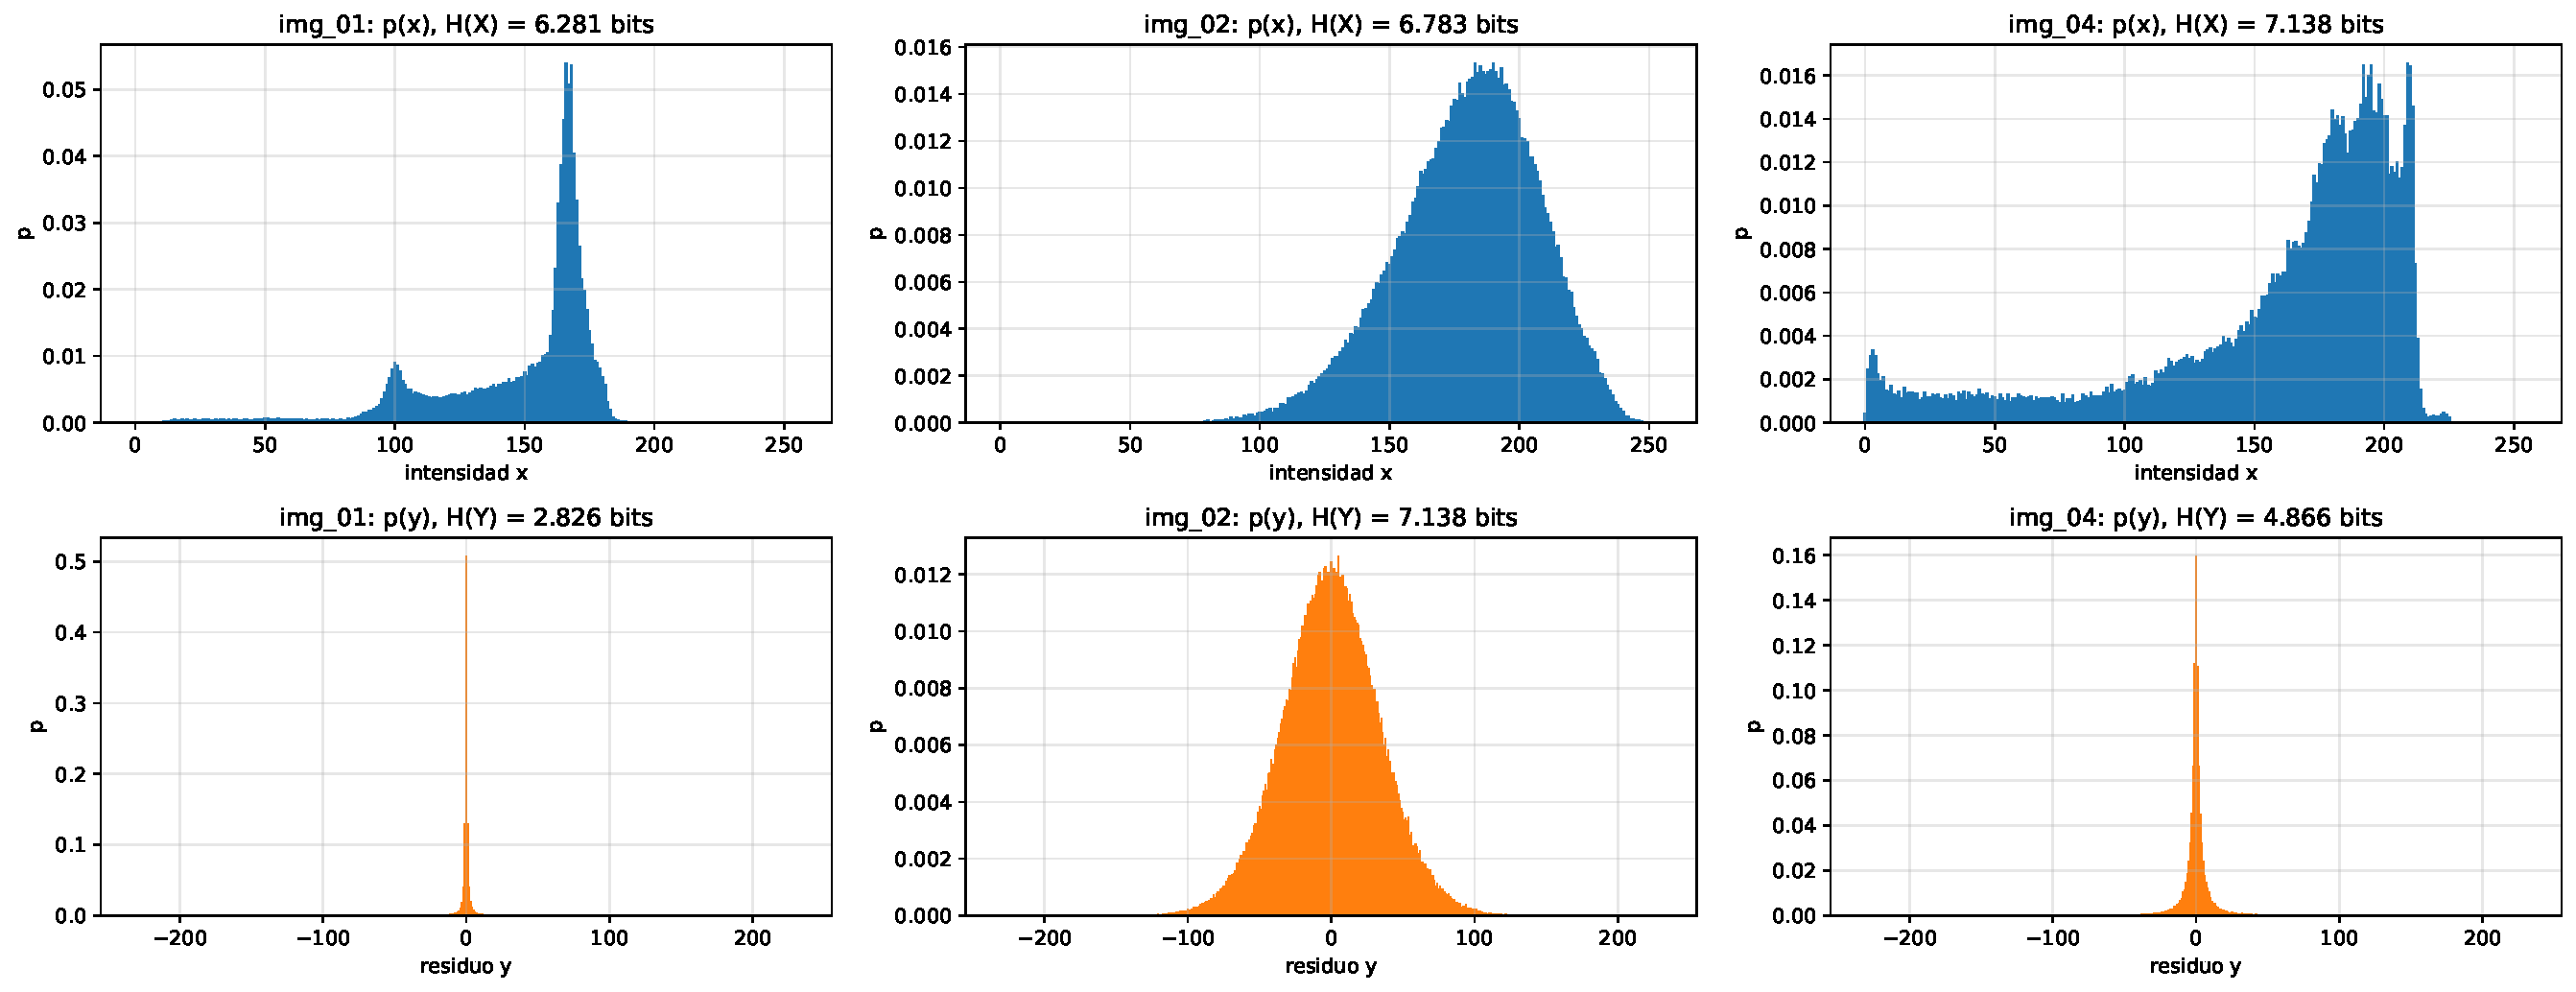
\includegraphics[width=\textwidth]{pmf_x_y}
  \caption{Fila superior: pmf empírica de las intensidades $\hat p(x)$ de cada imagen. Fila inferior:
  pmf empírica de los residuos $\hat p(y)$ sobre el alfabeto $\{-255,\dots,255\}$. Notar las escalas
  verticales: en \img{01} el residuo nulo concentra la mitad de la masa.}
  \label{fig:pmf}
\end{figure}

% =====================================================================
\section{Ejercicio 2: codificación diferencial}
% =====================================================================
\subsection{Masa de probabilidad y entropía de los residuos (inciso a)}
La fila inferior de la Figura~\ref{fig:pmf} y la Figura~\ref{fig:zoom} muestran $\hat p(y)$, y la
Tabla~\ref{tab:ej2a} compara las entropías. El comportamiento no es el mismo en las tres imágenes.

\begin{table}[H]
  \centering
  \caption{Entropía de las intensidades y de los residuos, cantidad de residuos distintos y fracción de
  residuos con $|y| \le 5$.}
  \label{tab:ej2a}
  \begin{tabular}{lrrrrr}
    \toprule
    Imagen & $H(X)$ [bits] & $H(Y)$ [bits] & $H(X) - H(Y)$ & Residuos distintos & $\hat\Prob(|Y| \le 5)$ \\
    \midrule
    \img{01} & 6.281 & 2.826 & $3.455$  & 230 & 0.925 \\
    \img{02} & 6.783 & 7.138 & $-0.355$ & 303 & 0.134 \\
    \img{04} & 7.138 & 4.866 & $2.272$  & 311 & 0.719 \\
    \bottomrule
  \end{tabular}
\end{table}

En \img{01} y \img{04} la pmf de los residuos se concentra alrededor de $y=0$: el
92.5\,\% y el 71.9\,\% de los residuos, respectivamente, caen en $|y|\le5$. Por eso $H(Y)$ es bastante
menor que $H(X)$, aun cuando el alfabeto de $Y$ (511 símbolos posibles, de los cuales aparecen entre
230 y 311) tiene casi el doble de símbolos que el de $X$. Es la redundancia espacial: como los píxeles vecinos
tienen intensidades parecidas, su diferencia es pequeña y mucho más predecible que el valor absoluto.

En \img{02} ocurre lo contrario: $H(Y)$ supera a $H(X)$. Solo el 13.4\,\% de los residuos cae en
$|y|\le5$. Las diferencias están más repartidas y el predictor basado en el vecino anterior no
reduce la entropía. En el inciso (c) se mide la dependencia entre esos mismos vecinos.

\begin{figure}[H]
  \centering
  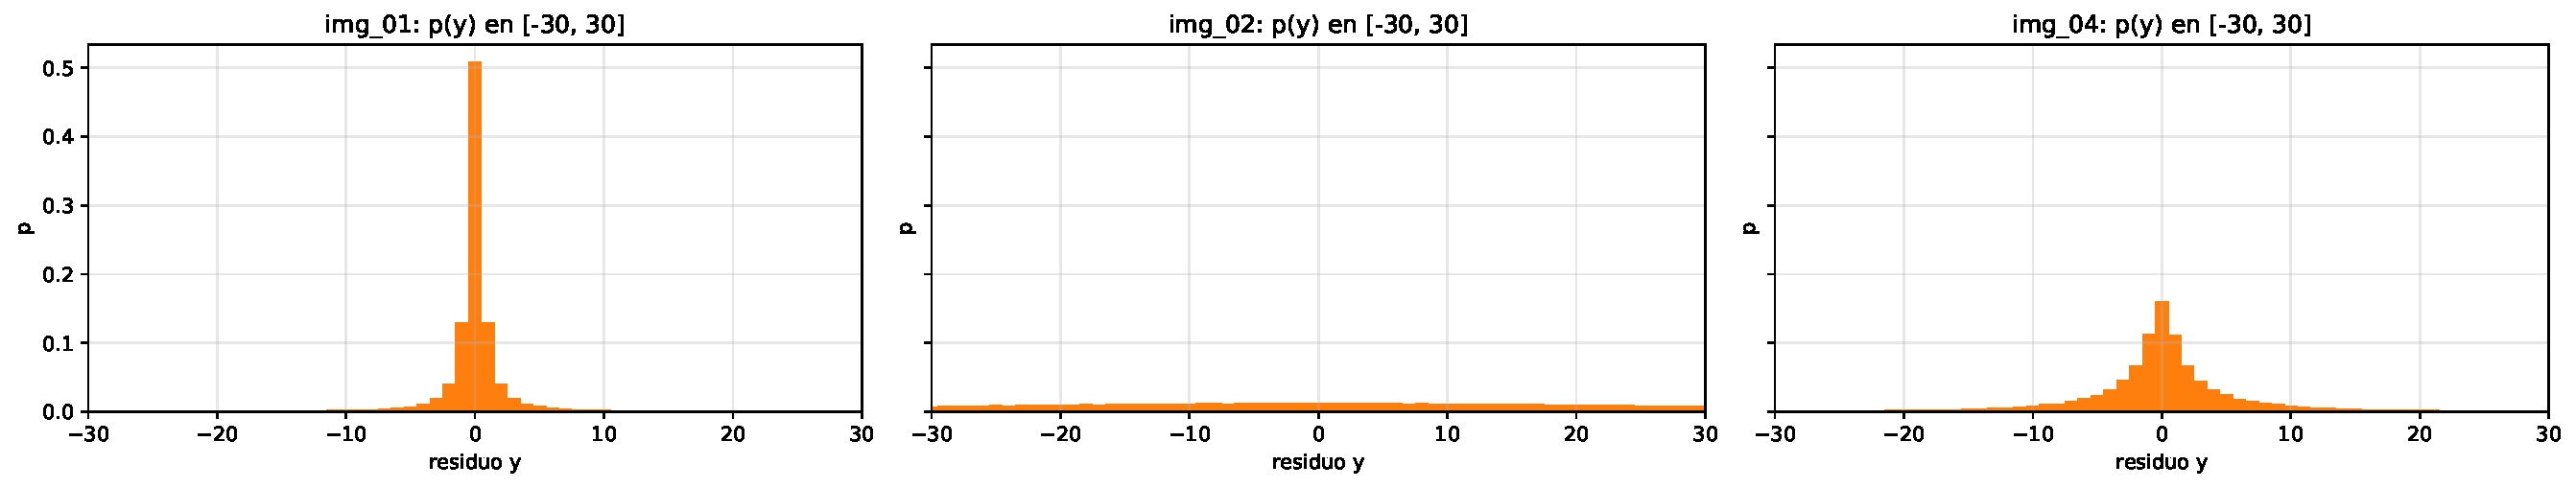
\includegraphics[width=\textwidth]{pmf_y_zoom}
  \caption{Detalle de $\hat p(y)$ en $[-30, 30]$. En \img{01} y \img{04} casi toda la masa está en
  unos pocos residuos alrededor de cero; en \img{02} la pmf es ancha incluso en esta ventana.}
  \label{fig:zoom}
\end{figure}

\subsection{Compresión de los residuos (inciso b)}
Aplicamos el mismo procedimiento del Ejercicio~1 sobre la fuente $Y$, con alfabeto
$\{-255,\dots,255\}$. La Tabla~\ref{tab:ej2b} muestra que los bits promedio medidos vuelven a
coincidir con la longitud media teórica $L_Y$ y que se cumple $H(Y) \le L_Y < H(Y) + 1$ en las tres
imágenes. Para comparar de manera justa con el Ejercicio~1 contamos también los 8 bits del píxel
inicial. El costo total por píxel es $(8+(MN-1)L_Y)/(MN)$; la diferencia con $L_Y$ es menor de
0.00005 en estas imágenes. Las tablas y los demás metadatos se cuentan en el Ejercicio~4.

\begin{table}[H]
  \centering
  \caption{Codificación de los residuos con Huffman y comparación con la codificación píxel a píxel.
  La tasa se calcula respecto de los 8 bits por píxel de la representación directa.}
  \label{tab:ej2b}
  \begin{tabular}{lrrrrrr}
    \toprule
    Imagen & $H(Y)$ & $L_Y$ & Bits/res. medidos & $L_X$ & Tasa directa & Tasa residuos \\
    \midrule
    \img{01} & 2.826 & 2.840 & 2.840 & 6.310 & 1.27 & 2.82 \\
    \img{02} & 7.138 & 7.179 & 7.179 & 6.809 & 1.17 & 1.11 \\
    \img{04} & 4.866 & 4.894 & 4.894 & 7.165 & 1.12 & 1.63 \\
    \bottomrule
  \end{tabular}
\end{table}

La Figura~\ref{fig:barras} resume los dos esquemas. En \img{01} la tasa de compresión pasa de 1.27 a
2.82 y en \img{04} de 1.12 a 1.63: como $\hat p(y)$ está concentrada en pocos símbolos, Huffman asigna
palabras más cortas a los residuos más frecuentes. Para $|y|\le 5$, las longitudes van de 1 a 7 bits
en \img{01} y de 3 a 5 bits en \img{04}. En \img{02} la
codificación de residuos es peor que la píxel a píxel ($L_Y = 7.18$ frente a $L_X = 6.81$), aunque
sigue por debajo de 8 bits porque la pmf de los residuos conserva cierta concentración alrededor de
cero. En ambos esquemas la longitud media de Huffman queda a menos de 0.05 bits de la entropía.
Las diferencias de compresión se explican principalmente por las distribuciones que se codifican.

\begin{figure}[H]
  \centering
  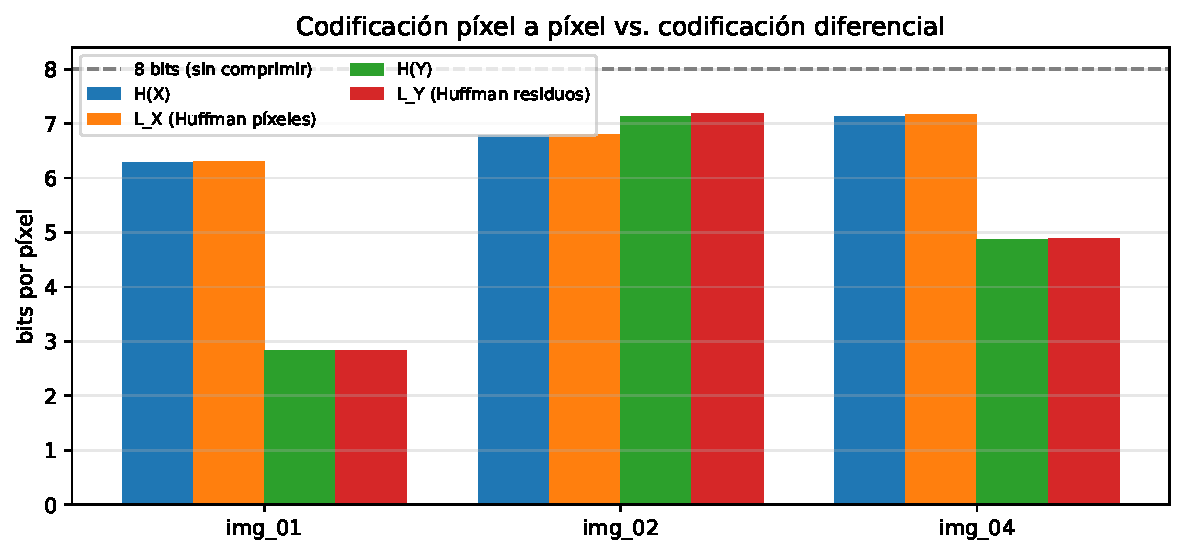
\includegraphics[width=0.78\textwidth]{barras_ej2}
  \caption{Entropía y longitud media del código de Huffman para las intensidades ($H(X)$, $L_X$) y
  para los residuos ($H(Y)$, $L_Y$), en bits por símbolo de cada fuente. La línea indica los 8 bits
  por píxel de la representación directa.}
  \label{fig:barras}
\end{figure}

\subsection{Información mutua entre píxeles vecinos (inciso c)}
La Figura~\ref{fig:conjunta} muestra la pmf conjunta $\hat p(x,x')$ en escala logarítmica para
visualizar probabilidades de distintos órdenes de magnitud. La diagonal $x=x'$ corresponde al
residuo nulo; las líneas $x-x'=y$ agrupan los pares que producen el mismo residuo. La
Tabla~\ref{tab:ej2c} resume la información mutua y las entropías relacionadas.

\begin{table}[H]
  \centering
  \caption{Entropías e información mutua empíricas en bits. El cociente $\MI/H(X)$ es adimensional.}
  \label{tab:ej2c}
  \begin{tabular}{lrrrrrrr}
    \toprule
    Imagen & $H(X)$ & $H(X,X')$ & $\MI$ & $\MI / H(X)$ & $H(X \mid X')$ & $H(Y)$ & $H(X) - H(Y)$ \\
    \midrule
    \img{01} & 6.281 &  8.840 & 3.722 & 0.59 & 2.559 & 2.826 & $3.455$ \\
    \img{02} & 6.783 & 13.450 & 0.116 & 0.02 & 6.667 & 7.138 & $-0.355$ \\
    \img{04} & 7.138 & 11.496 & 2.779 & 0.39 & 4.358 & 4.866 & $2.272$ \\
    \bottomrule
  \end{tabular}
\end{table}

\begin{figure}[H]
  \centering
  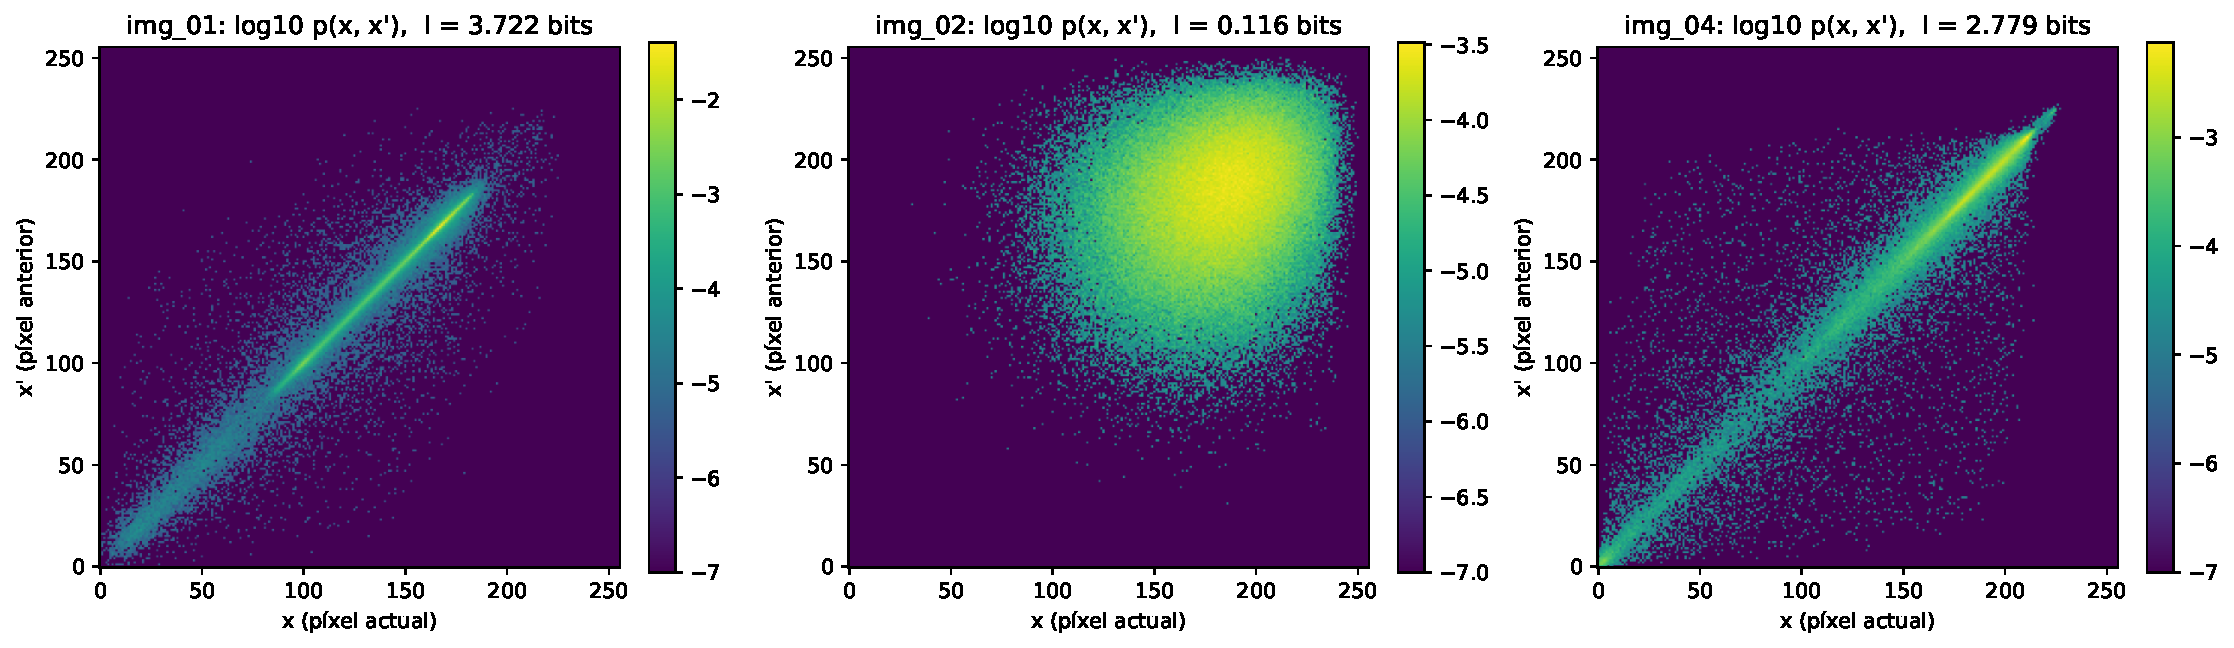
\includegraphics[width=\textwidth]{pmf_conjunta}
  \caption{Pmf conjunta $\hat p(x, x')$ del píxel actual $x$ y su vecino anterior $x'$, en escala
  $\log_{10}$. Las celdas sin ocurrencias se muestran en el color más oscuro.}
  \label{fig:conjunta}
\end{figure}

En \img{01} la masa se concentra cerca de la diagonal, especialmente entre 100 y 190. La
información mutua estimada es 3.72 bits y representa el 59\,\% de $H(X)$ para estos pares. En
\img{04} también se observa la diagonal, pero con mayor dispersión; la reducción relativa es del
39\,\%. Aun conociendo el vecino, quedan 2.56 y 4.36 bits de entropía condicional, respectivamente.
En \img{02} la nube es más difusa y la información mutua estimada es mucho menor: 0.116 bits.

En las tres imágenes se verifica $H(Y)\ge H(X\mid X')$. La diferencia es de 0.27 bits en
\img{01} y de 0.51 en \img{04}: los residuos aprovechan buena parte de la dependencia entre estos
vecinos. En \img{02}, en cambio, $H(X)-H(Y)<0$ y la resta empeora la compresión. Estos valores se
estiman con histogramas finitos; una información mutua estimada positiva no basta por sí sola para
afirmar dependencia de una fuente subyacente, ni un valor pequeño demuestra independencia.

% =====================================================================
\section{Ejercicio 3: interpretación de los resultados}
% =====================================================================
\paragraph{(a) Diferencias de entropía entre imágenes.}
Las tres imágenes contienen un número similar de niveles de gris distintos: 224 en \img{01},
205 en \img{02} y 228 en \img{04}. La frecuencia con la que aparece cada nivel varía entre imágenes. En
\img{01} predominan unos pocos tonos de las dunas; en \img{02} la masa se reparte en una campana
más ancha; en \img{04} las intensidades están más repartidas y la entropía es la mayor.
$H(X)$ depende de las probabilidades de los niveles, no de su separación ni del orden de los
píxeles. Por eso no es una medida directa de contraste o textura: una permutación de las posiciones
conserva exactamente el histograma y la entropía.

\paragraph{(b) Qué representa la información mutua.}
$\MI$ cuantifica cuánto se reduce la incertidumbre sobre el píxel actual al conocer el vecino
anterior del recorrido. En estas imágenes es mayor en las dunas, menor en la partitura y muy baja
en la textura de arena. Las regiones suaves generan muchos pares próximos a la diagonal; los
bordes y la textura dispersan esos pares. La información mutua mide dependencia en general, no
necesariamente semejanza de intensidades. Tampoco describe toda la estructura espacial: aquí solo
se consideran los vecinos de la serpentina.

\paragraph{(c) Compresión píxel a píxel frente a compresión de residuos.}
En las dunas y la partitura, los residuos pequeños son frecuentes y requieren menos bits en
promedio que las intensidades. Las tasas de compresión pasan de 1.27 a 2.82 y de 1.12 a 1.63.
En la textura de arena ocurre lo contrario: los residuos requieren 7.18 bits por símbolo frente
a los 6.81 de las intensidades, por lo que conviene la codificación directa.

La desigualdad $H(Y)\ge H(X\mid X')$ acota la mejora posible, pero una información mutua alta no
la garantiza. Una secuencia alternante 0,255,0,255 tiene dependencia casi perfecta y residuos que
alternan $+255$ y $-255$; ambos códigos usan un bit por símbolo. La identidad
$H(X)-H(Y)=\MI-I(Y;X')$ muestra que el ahorro depende de cuánto aprovecha la resta la dependencia
disponible. Para comparar longitudes Huffman se suman además las redundancias de los códigos.

% =====================================================================
\section{Experimento adicional: píxeles mezclados}
% =====================================================================
Para distinguir el efecto del histograma del efecto del orden espacial, permutamos los píxeles de
\img{01} sin cambiar sus valores ni las dimensiones. Usamos una semilla fija (42) y repetimos los
cálculos sobre los vecinos de la nueva serpentina. Se comprobó que los histogramas y la cantidad de
bits de la codificación directa son exactamente iguales. La permutación se analiza como una imagen
nueva, sin proponerla como transformación del compresor.

\begin{figure}[!htbp]
  \centering
  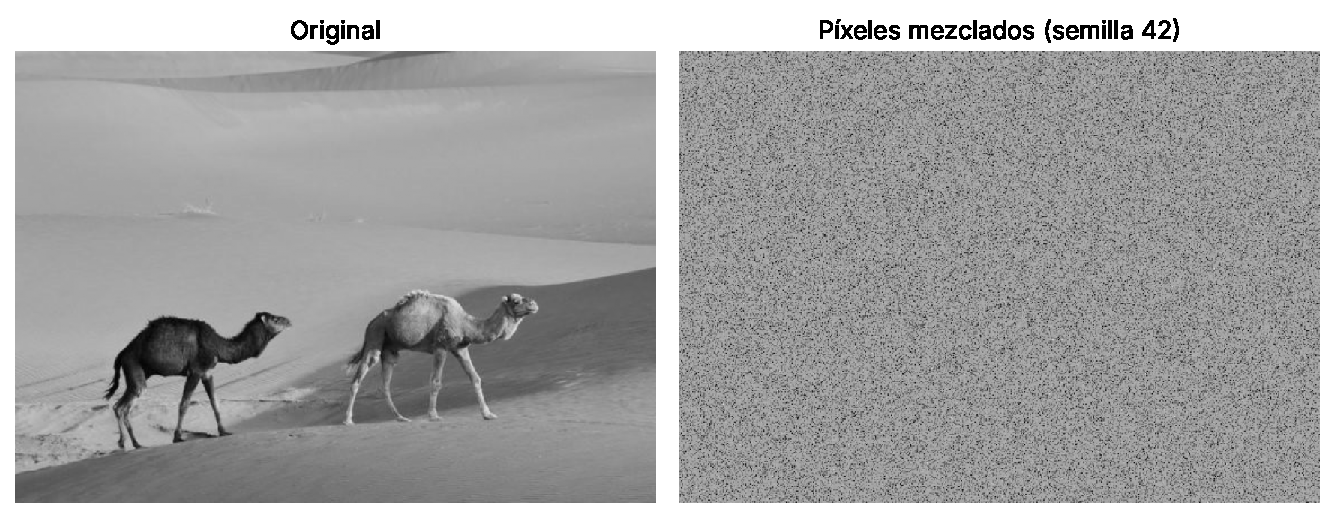
\includegraphics[width=0.85\textwidth]{mezclado}
  \caption{La imagen de dunas y una permutación de sus píxeles. Las frecuencias de las intensidades
  se conservan, pero se pierde la continuidad espacial.}
  \label{fig:mezclado}
\end{figure}

\begin{table}[!htbp]
  \centering
  \caption{Experimento con píxeles mezclados. $L_X$ está en bits por píxel y $L_Y$ en bits por residuo;
  las entropías y la información mutua, en bits.}
  \label{tab:mezclado}
  \begin{tabular}{lrrrrr}
    \toprule
    Versión & $H(X)$ & $L_X$ & $H(Y)$ & $L_Y$ & $\MI$ \\
    \midrule
    Original & 6.2809 & 6.3100 & 2.8262 & 2.8402 & 3.7217 \\
    Mezclada & 6.2809 & 6.3100 & 7.3711 & 7.3995 & 0.1055 \\
    \bottomrule
  \end{tabular}
\end{table}

La codificación directa cuesta lo mismo porque solo utiliza las frecuencias de las intensidades.
En cambio, al mezclar se pierde la continuidad de las dunas y aparecen diferencias grandes entre
vecinos con más frecuencia. La longitud media de los residuos sube de 2.84 a 7.40 bits y supera
los 6.31 bits por píxel de la codificación directa. El experimento muestra que la ventaja original de
los residuos depende de la disposición espacial, que el histograma de intensidades no registra.

La información mutua estimada baja mucho, pero no llega exactamente a cero. Se trata de una sola
permutación de un conjunto finito evaluada con histogramas empíricos. El experimento es ilustrativo
y no constituye una prueba estadística de independencia.

% =====================================================================
\section{Ejercicio 4: compresor y descompresor de línea de comando}
% =====================================================================
Implementamos dos programas en Python. El compresor recibe una imagen en un formato estándar (JPG o
PNG), la convierte a escala de grises, calcula los residuos sobre el recorrido en serpentina,
construye el código de Huffman y escribe un archivo binario con extensión \texttt{.tp2}. El
descompresor lee ese archivo, decodifica los residuos, reconstruye la imagen por suma acumulada y la
muestra en pantalla; opcionalmente la guarda y la compara píxel a píxel con la original.

El archivo contiene todo lo que el decodificador necesita y no puede deducir: una firma de 4 bytes,
las dimensiones (dos enteros de 32 bits), el píxel inicial (1 byte), la cantidad de símbolos de la
tabla (2 bytes), la tabla propiamente dicha (por cada residuo que aparece, su valor en 2 bytes y la
longitud de su palabra de código en 1 byte), la cantidad de bits útiles (8 bytes) y, por último, un
único flujo de bits con las palabras de código concatenadas en el orden de la tabla seguidas de los
residuos codificados, completado con ceros hasta el byte. Cada entrada fija de la tabla ocupa
3 bytes; las palabras de código también se guardan, al comienzo del flujo de bits. Incluyendo esas
palabras, los metadatos ocupan aproximadamente entre 1.1 y 1.4\,KB en estas imágenes.

\begin{table}[H]
  \centering
  \caption{Resultados del compresor sobre las tres imágenes. El tamaño original corresponde a la
  imagen en escala de grises a 8 bits por píxel; el comprimido incluye el encabezado. En los tres casos
  el descompresor reconstruye exactamente la imagen original.}
  \label{tab:ej4}
  \begin{tabular}{lrrrr}
    \toprule
    Imagen & Bits/píxel (datos) & Original [B] & Comprimido [B] & Tasa \\
    \midrule
    \img{01} & 2.840 & 227\,200 &  81\,763 & 2.78 \\
    \img{02} & 7.179 & 249\,696 & 225\,407 & 1.11 \\
    \img{04} & 4.894 &  72\,128 &  45\,543 & 1.58 \\
    \bottomrule
  \end{tabular}
\end{table}

Los valores coinciden con los del Ejercicio~2 a la precisión mostrada. Las tasas del archivo son
algo menores porque incluyen todos los metadatos. Verificamos que las tres reconstrucciones son idénticas a las
originales en escala de grises. Para \img{02} el programa comprime, pero un compresor que probara
ambos esquemas y guardara en el encabezado cuál usó obtendría un archivo más chico codificando las
intensidades directamente.

% =====================================================================
\section{Conclusiones}
Huffman produjo longitudes medias a menos de 0.05 bits de las entropías estimadas, y las cuentas
teóricas coincidieron con los bits medidos. La codificación por residuos mejoró las tasas de las
dunas y la partitura, pero empeoró la de la textura de arena. Por eso conviene evaluar el predictor
sobre cada imagen: la dependencia entre vecinos no garantiza que la resta reduzca la entropía.

El experimento con píxeles mezclados permitió separar ambos efectos. El histograma y la compresión directa
se conservaron, mientras que los residuos perdieron su ventaja al cambiar el orden espacial. En la
implementación hubo que tratar por separado el caso de un único símbolo: asignarle la palabra
\texttt{0} permitió conservar el número de ocurrencias con el decodificador provisto. Las tres
imágenes originales se recuperaron exactamente desde los archivos \texttt{.tp2}. Como continuación
se podría comparar la serpentina horizontal con una vertical, especialmente en la partitura.

% =====================================================================
{\small
\begin{thebibliography}{9}
\bibitem{tp2} Cátedra de I206 -- Inferencia y Estimación (2026). \emph{Trabajo práctico 2: Compresión
  de imágenes sin pérdida mediante codificación de Huffman} y funciones auxiliares
  \texttt{huffman\_code} y \texttt{huffman\_decode}. Universidad de San Andrés.
\bibitem{teoricas} Material teórico de I206 -- Inferencia y Estimación (2026): \emph{Teoría de la
  información -- Definiciones}. Universidad de San Andrés.
\bibitem{teoricas2} Material teórico de I206 -- Inferencia y Estimación (2026): \emph{Teoría de la
  información -- Información mutua -- Fisher}. Universidad de San Andrés.
\bibitem{shannon} Shannon, C. E. (1948). A Mathematical Theory of Communication. \emph{Bell System
  Technical Journal}, 27, 379--423 y 623--656.
\bibitem{huffman} Huffman, D. A. (1952). A Method for the Construction of Minimum-Redundancy Codes.
  \emph{Proceedings of the IRE}, 40(9), 1098--1101.
\bibitem{cover} Cover, T. M. y Thomas, J. A. (2006). \emph{Elements of Information Theory} (segunda
  edición). Wiley. Capítulos 2 y 5.
\end{thebibliography}
}

\end{document}
